\subsection{Checkout - Payment}

%For the main pages put a mockup and describe it in detail.

%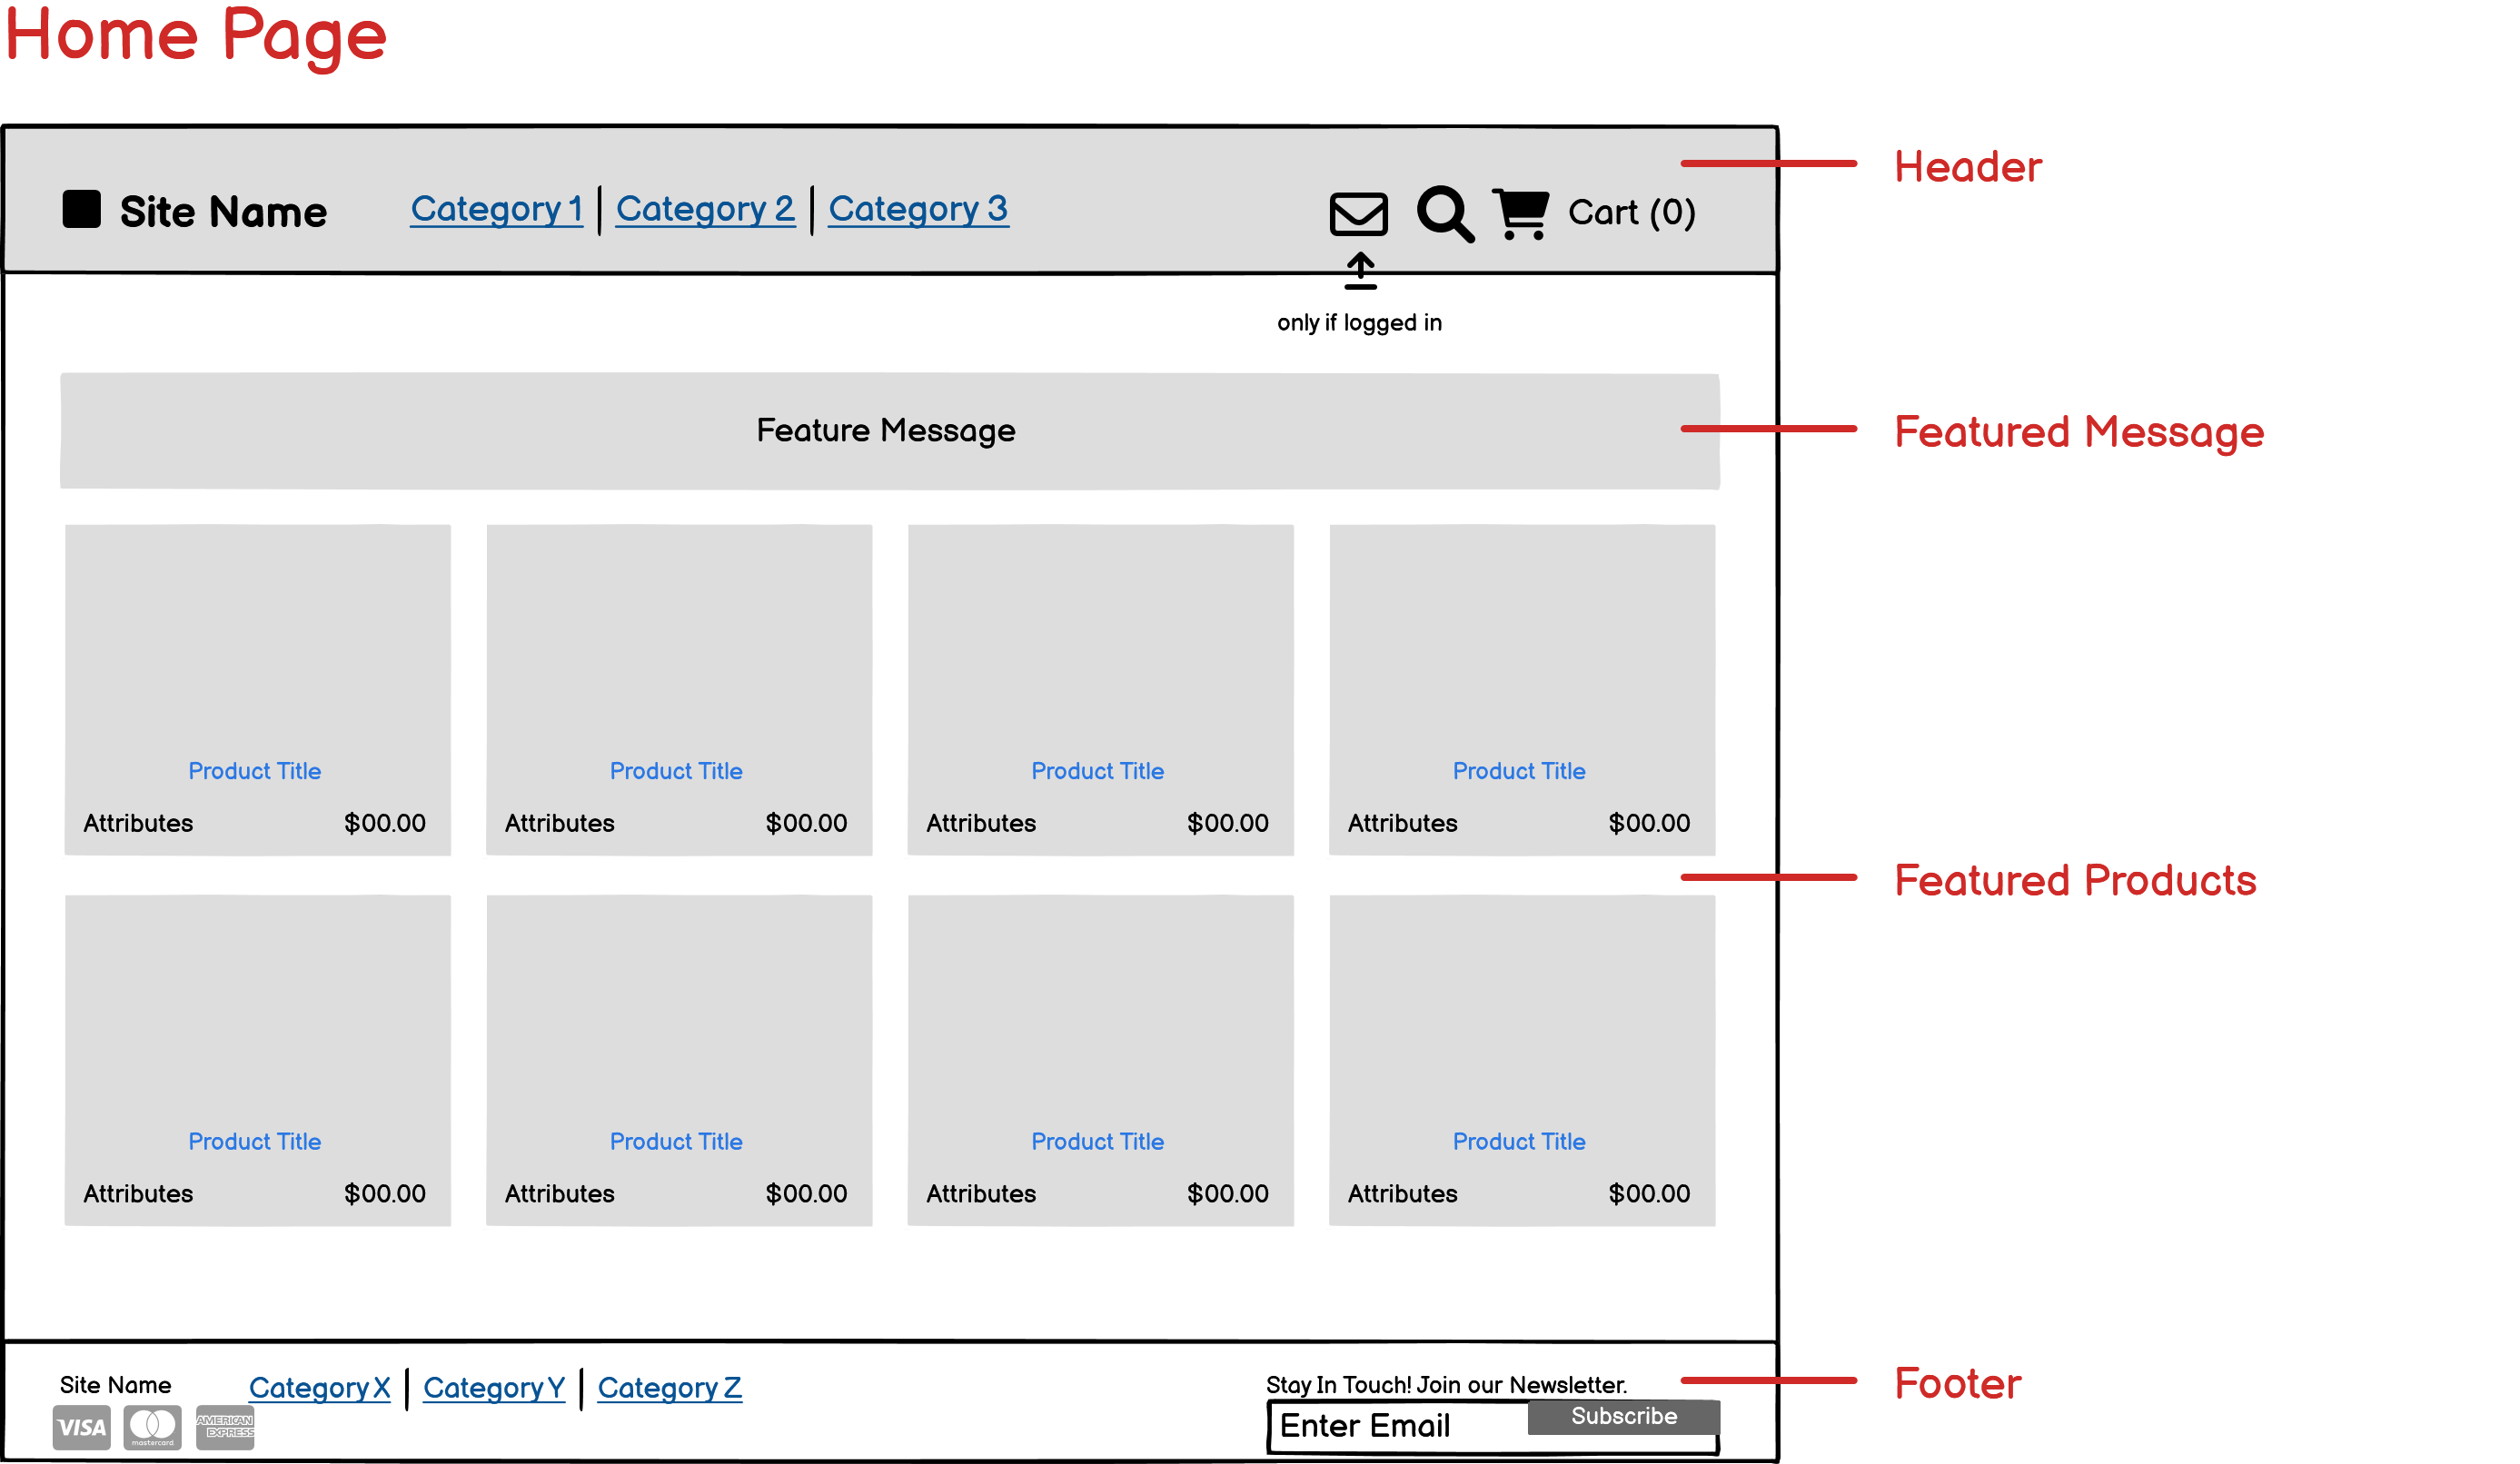
\includegraphics[scale=0.5]{logos/Images/pages/Home Page.png}

\begin{figure}[h]
    \centering
    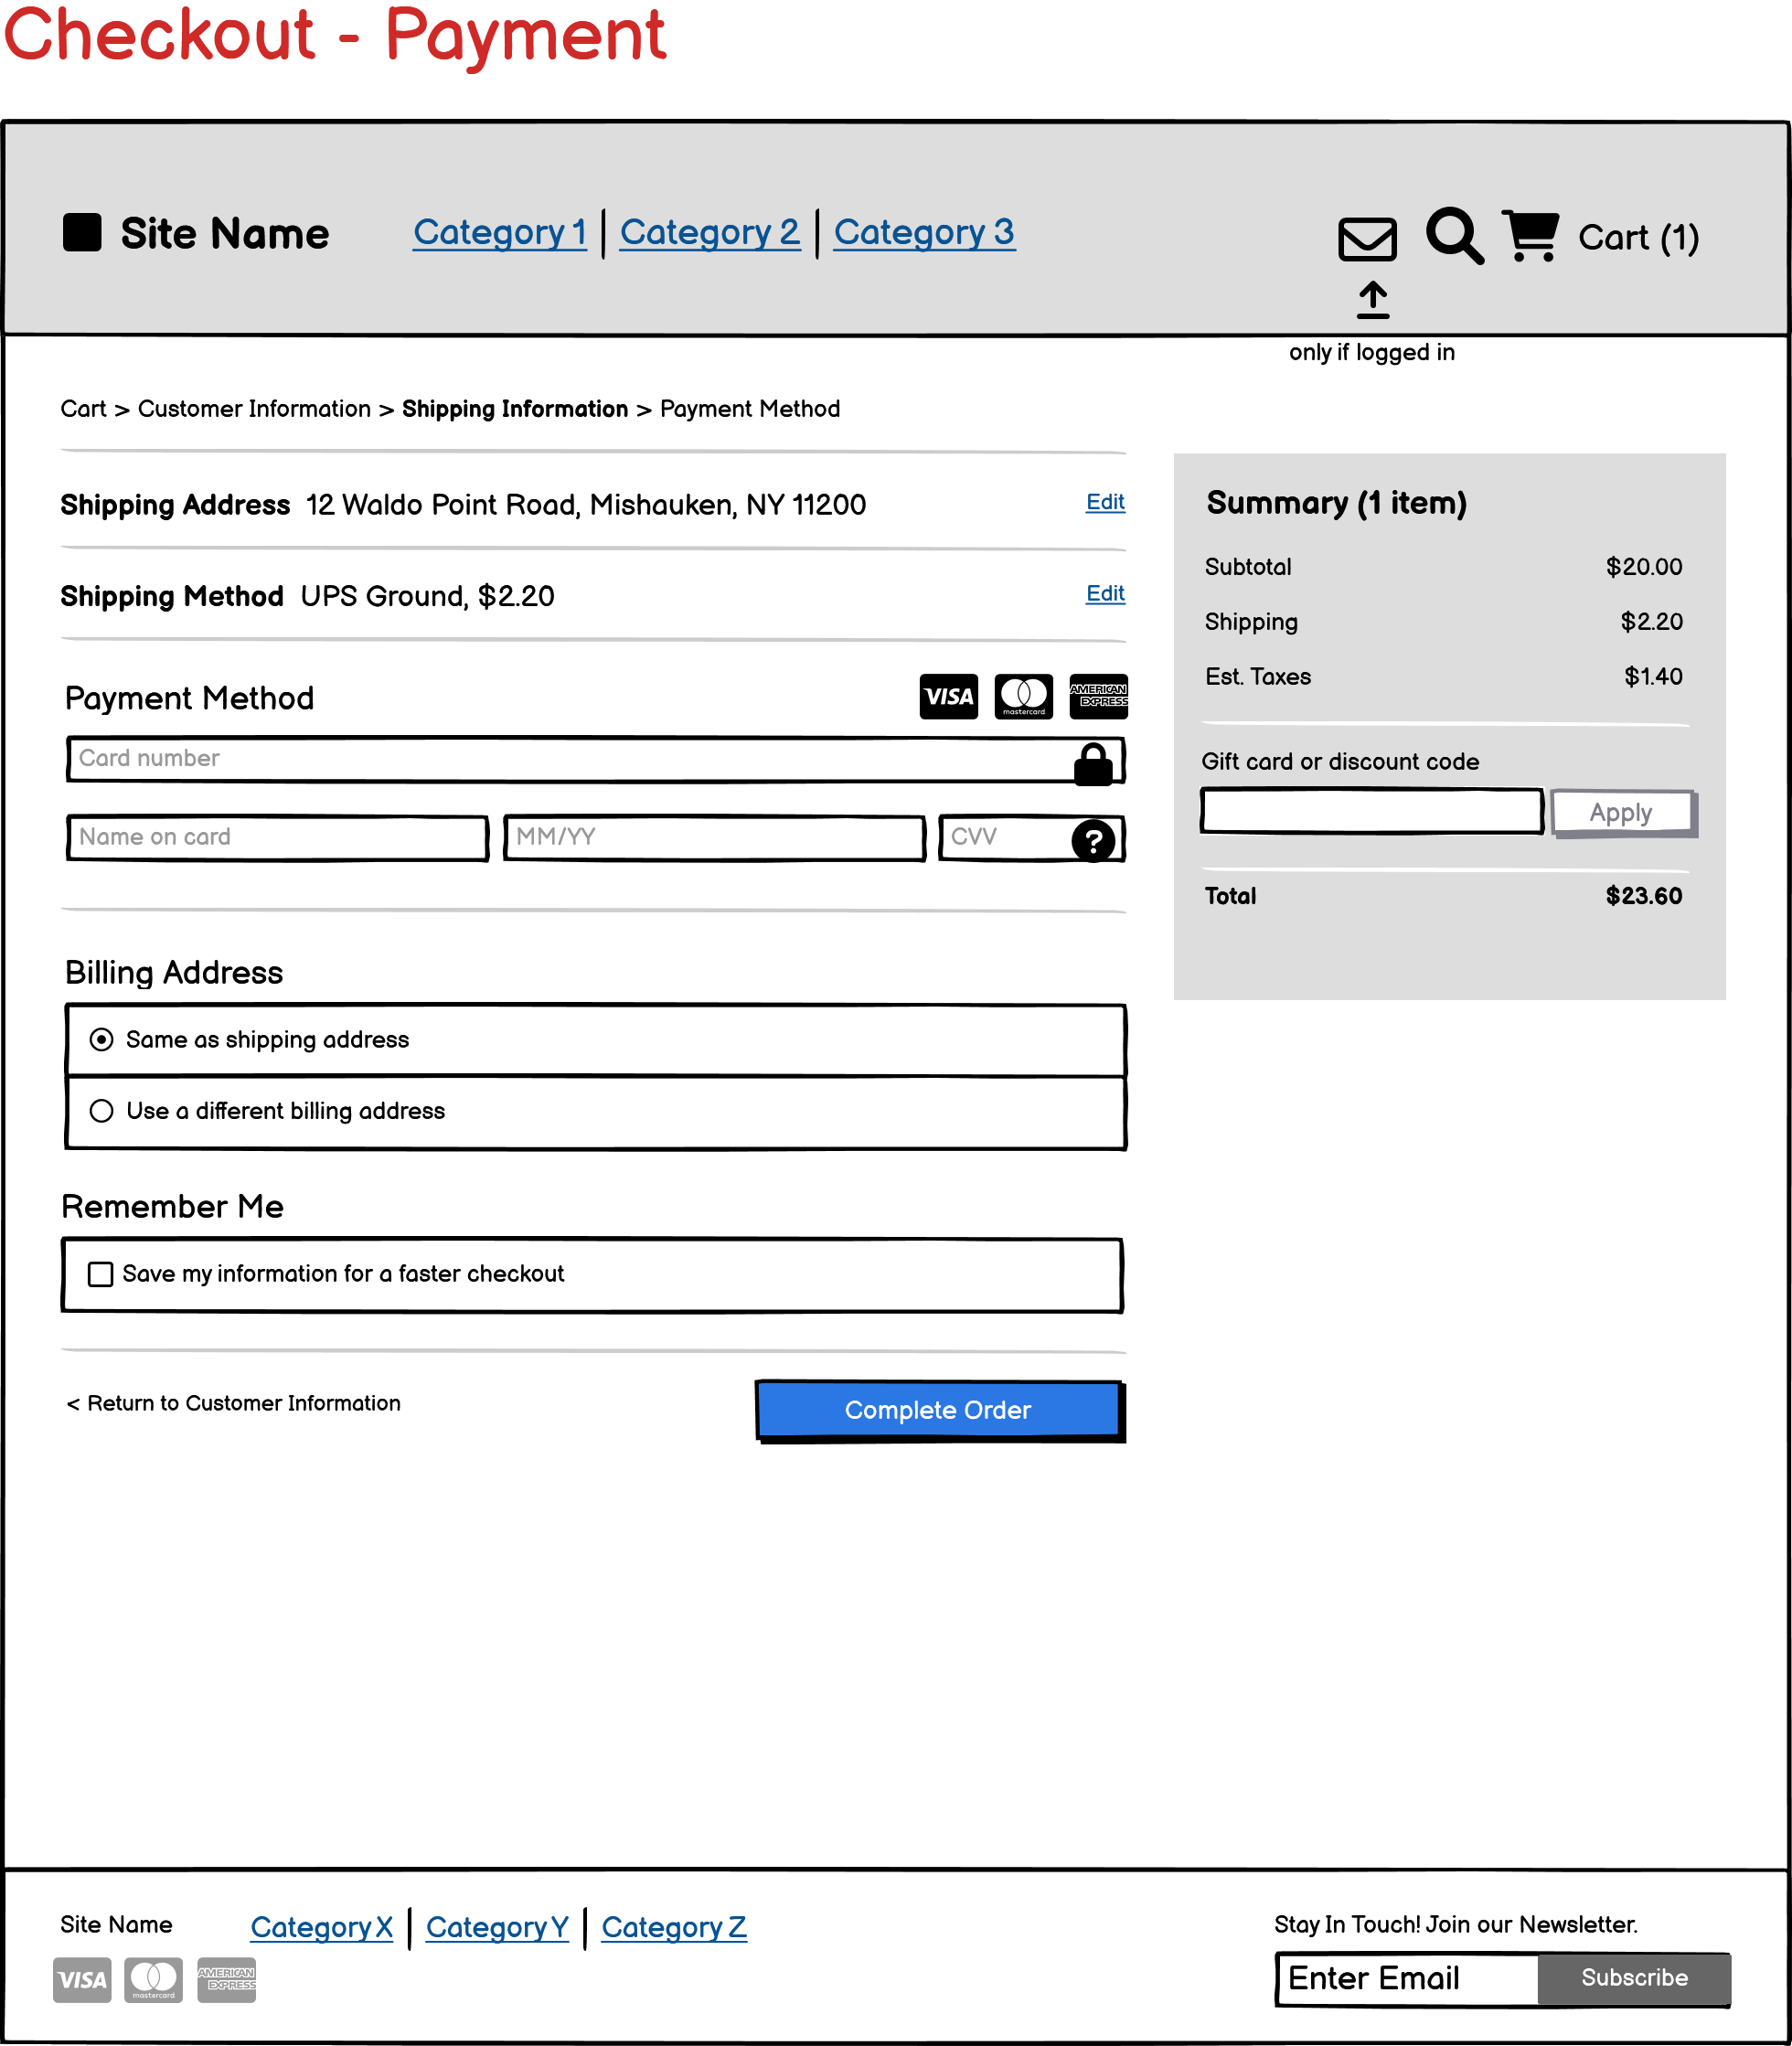
\includegraphics[scale=0.4]{logos/Images/pages/Checkout - Payment.png}
    \caption{Checkout - Payment}
    \label{fig:my_label}
\end{figure}
\hfill \break
After the user has selected the delivery address and the delivery service on the delivery method page, he will be redirected to the payment page.\\\\
On the payment page, the user can select the desired payment method and enter the credit card details. Here the user can also specify whether the billing address is the same as the delivery address or not.\\\\
Once all the required information has been entered, the user can complete the order by clicking on the submit button. Once the payment has been processed, the user will be redirected to an order confirmation page.\\\\
The payment page is an important page for the successful completion of an order. It provides the user with an easy and secure way to pay for their order and ensures that the transaction is smooth and secure.